\chapter{Appendix}
\begin{table}[htbp]
    \centering
    \begin{tabular}{c|c c c|c c c}
        \toprule
        {}&\multicolumn{3}{c}{$0\, fj$ region}&\multicolumn{3}{c}{$\geq 1\, fj$ region}\\
        Event parameter &  Background &  $tq\gamma$ &  Data &  Background &  $tq\gamma$ &  Data \\
        \midrule
        top\_m                            & -0.51 &      0.01 &   0.03 & -0.41 &      0.06 &   0.04 \\ \hline
        Wbsn\_e                           & -0.35 &     -0.02 &   0.00 & -0.38 &      0.00 &  -0.00 \\ \hline
        blep\_m                           & -0.39 &      0.01 &   0.01 & -0.33 &      0.02 &   0.01 \\ \hline
        topph\_ctheta                     & -0.28 &     -0.00 &     & -0.33 &     -0.01 &   0.02 \\ \hline
        transMassWb                      & -0.47 &     -0.00 &     & -0.33 &     -0.02 &  -0.02 \\ \hline
        lep1\_pt                          & -0.36 &        &     & -0.32 &      0.54 &   0.43 \\ \hline
        HT                               & -0.21 &     -0.24 &  -0.35 & -0.30 &     -0.22 &  -0.32 \\ \hline
        met\_met                          & -0.26 &     -0.05 &   0.02 & -0.26 &      0.00 &  -0.01 \\ \hline
        topph\_pt                         & -0.02 &     -0.12 &  -0.14 & -0.18 &     -0.06 &  -0.03 \\ \hline
        blep\_dr                          & -0.15 &     -0.06 &  -0.14 & -0.14 &     -0.05 &  -0.07 \\ \hline
        bph\_pt                           & -0.08 &     -0.03 &   0.02 & -0.13 &      0.00 &   0.02 \\ \hline
        transMassWph                     & -0.17 &      0.00 &  -0.00 & -0.10 &      0.00 &   0.02 \\ \hline
        fjph\_dr                          &  0.00 &      0.18 &   0.19 & -0.06 &      0.14 &   0.15 \\ \hline
        lbj\_pt                           & -0.12 &     -0.32 &  -0.50 & -0.05 &     -0.24 &  -0.42 \\ \hline
        fjph\_deta                        &  0.00 &     -0.36 &  -0.29 & -0.03 &     -0.29 &  -0.33 \\ \hline
        fj\_phi                           & -0.00 &     -0.09 &  -0.08 & -0.03 &     -0.11 &  -0.19 \\ \hline
        lep1\_eta                         &  0.02 &     -0.30 &  -0.37 & -0.02 &     -0.28 &  -0.39 \\ \hline
        met\_phi                          &  0.00 &      0.27 &   0.14 & -0.01 &      0.25 &   0.18 \\ \hline
        lep1\_id                          & -0.16 &     -0.27 &  -0.43 & -0.00 &     -0.20 &  -0.35 \\ \hline
        ph\_eta                           &  0.00 &        &     &  0.00 &      0.45 &   0.22 \\ \hline
        ph\_phi                           & -0.00 &     -0.05 &  -0.09 &  0.01 &     -0.08 &  -0.13 \\ \hline
        fj\_eta                           & -0.00 &        &     &  0.01 &     -0.05 &  -0.01 \\ \hline
        lbj\_phi                          & -0.00 &      0.07 &   0.03 &  0.01 &      0.45 &   0.28 \\ \hline
        lbj\_eta                          &  0.02 &     -0.02 &   0.00 &  0.02 &     -0.16 &  -0.09 \\ \hline
        fjph\_m                           &    &     -0.02 &   0.00 &  0.04 &     -0.16 &  -0.08 \\ \hline
        ph\_pt                            &  0.06 &        &     &  0.08 &      0.29 &   0.14 \\ \hline
        fjph\_ctheta                      &    &      0.25 &   0.15 &  0.08 &      0.12 &   0.12 \\ \hline
        lepph\_dr                         &  0.10 &     -0.03 &  -0.19 &  0.11 &     -0.01 &  -0.14 \\ \hline
        lbj\_tagWeightBin &  0.12 &     -0.16 &  -0.21 &  0.13 &     -0.17 &  -0.25 \\ 
        \_DL1r\_Continuous &&&&&&\\ \hline
        bfj\_m                            &    &      0.02 &  -0.00 &  0.19 &     -0.01 &   0.00 \\ \hline
        bph\_m                            &  0.19 &     -0.20 &  -0.24 &  0.25 &     -0.26 &  -0.34 \\ \hline
        fjph\_e                           &  0.04 &     -0.07 &  -0.13 &  0.27 &     -0.03 &  -0.10 \\ \hline
        fjet\_flag                        &    &     -0.28 &  -0.42 &  0.37 &     -0.19 &  -0.31 \\ \hline
        \bottomrule
        \end{tabular}
    \caption{List of correlations between samples and the NN output in the zero forward jet region as well as samples in the $\geq 1$ forward jet region.}
    \label{tab:corrAll}
\end{table}
\begin{figure}[htbp]
    \centering
    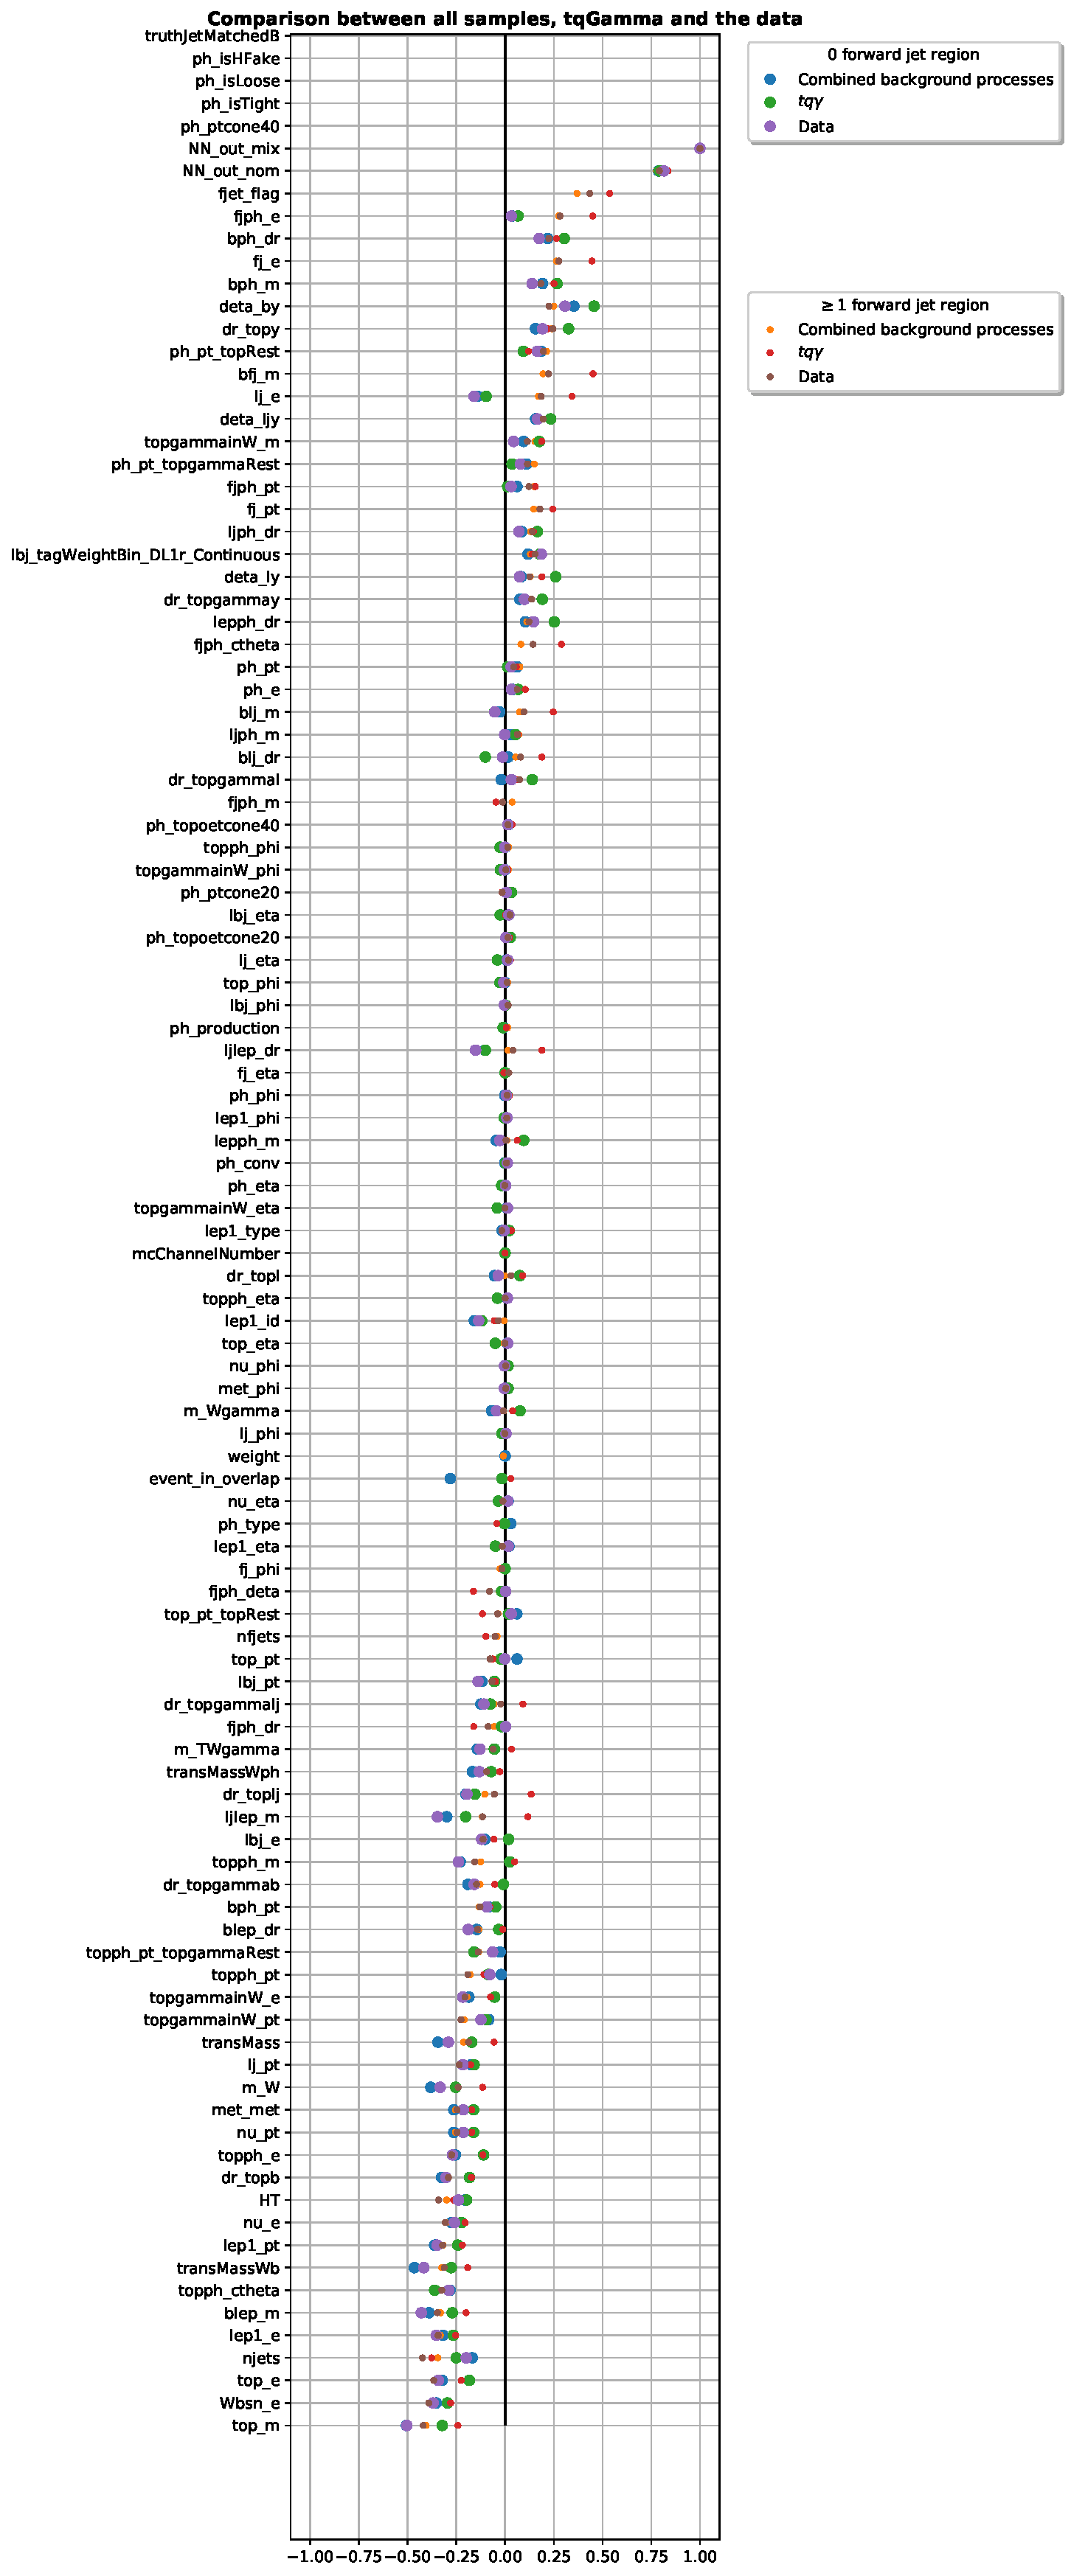
\includegraphics[width=0.7\textwidth]{Plots/corrAll.pdf}
    \caption{Correlations of all event properties with the NN output in the $0\,fj$ and $\geq 1\,fj$ region for the background samples, $tq\gamma$ and the measured data.}
    \label{fig:corrAll}
\end{figure}